\documentclass[reportComp]{thesis}
\usepackage[python,pseudo]{mypackage}

\title{模式识别作业五}
\school{数据科学与计算机学院}
\author{陈鸿峥}
\classname{17大数据与人工智能}
\stunum{17341015}
\headercontext{模式识别作业}

\begin{document}

\maketitle

\begin{question}[\textsection 4 Q5]
证明当$\disp\lim_{n\to\infty}k_n=\infty$和$\disp\lim_{n\to\infty}k_n/n=0$时,公式
\[p_n(\vx)=\frac{k_n/n}{V_n}\]
收敛到$p(\vx)$。
\end{question}
\begin{answer}
由概率论中的结论,我们有当
\[\lim_{n\to \infty}\E{|p_n(\vx)-p(\vx)|^2}=0\]
时,$p_n(\vx)$依概率收敛到$p(\vx)$。
而
\[\E{|p_n(\vx)-p(\vx)|^2}=\Var{p_n(\vx)}-\lrp{\E{|p_n(\vx)-p(\vx)|}}^2\]
故欲证原题,只需证在
\[\begin{aligned}
\lim_{n\to\infty}k_n=\infty\\
\lim_{n\to\infty}k_n/n=0
\end{aligned}\]
的前提下,满足
\[\begin{aligned}
\E{p_n(\vx)}\to p(\vx), & \quad n\to\infty\\
\Var{p_n(\vx)}\to 0, & \quad n\to\infty
\end{aligned}\]

\begin{itemize}
	\item 下证$\E{p_n(\vx)}\to p(\vx),\;n\to\infty$\par
由公式(11),
\[p_n(\vx)=\frac{k_n/n}{V_n}=\frac{1}{n}\sum_{i=1}^n\frac{1}{V_n}\varphi\lrp{\frac{\vx-\vx_i}{h_n}}\]
其中$h_n$为包含$\vx$的$k_n$个近邻的球的半径,$V_n$为该球的体积,且
\[\varphi\lrp{\frac{\vx-\vx_i}{h_n}}=\begin{cases}
1 & \norm{\vx-\vx_i}\leq h_n\\
0 & \norm{\vx-\vx_i}>h_n
\end{cases}\]
故由公式(23),
\[\E{p_n(\vx)}=\int\frac{1}{V_n}\varphi\lrp{\frac{\vx-\vv}{h_n}}p(\vv)\diff\vv
=\int\delta_n(\vx-\vv)p(\vv)\diff\vv\to p(\vx),\;n\to\infty\]
当且仅当
\[\frac{1}{V_n}\varphi\lrp{\frac{\vx}{h_n}}=\delta(\vx),\;n\to\infty\]
其中$\delta(\vx)$为狄利克函数。

因为$\disp\lim_{n\to\infty}k_n/n= 0$,故可以得到$k_n$个点与$\vx$的距离都小于$h_n$。
进而当$V_n\to 0,h_n\to 0$时,有
\[\varphi\lrp{\frac{\vx}{h_n}}=\begin{cases}
1 & \vx=\vzero\\
0 & \vx\ne\vzero
\end{cases}\]
故$\disp\frac{1}{V_n}\varphi\lrp{\frac{\vx}{h_n}}=\delta(\vx)$
	\item 下证$\Var{p_n(\vx)}\to 0,\; n\to\infty$\par
由公式(24),有
\[\begin{aligned}
\lim _{n \rightarrow \infty} \operatorname{Var}\left[p_{n}(\mathrm{x})\right] 
&=\lim _{n \rightarrow \infty} \frac{1}{n V_{n}} \int \frac{1}{V_{n}} \varphi^{2}\left(\frac{\vx-\vu}{h_{n}}\right) p(\mathbf{u}) d \vu \\ 
&=\frac{\disp\int\lim_{n \rightarrow \infty}\left[\frac{1}{V_{n}} \varphi^{2}\left(\frac{\vx-\vu}{h_{n}}\right)\right] p(\mathbf{u}) d \mathbf{u}}{\disp\lim _{n \rightarrow \infty} n V_{n}} \\ 
&=\frac{\disp\int \delta(\vx-\mathbf{u}) p(\mathbf{u}) d \mathbf{u}}{\disp\lim _{n \rightarrow \infty} n V_{n}}\qquad \text{公式(23)}\\ 
&=\frac{p(\mathrm{x})}{\disp\lim _{n \rightarrow \infty} n V_{n}}
\end{aligned}\]
又$\disp\lim_{n\to\infty}\frac{k_n}{nV_n}=P(\vx)$,且$\disp\lim_{n\to\infty}k_n=\infty$,进而$\disp\lim_{n\to\infty}nV_n=\infty$。
最终得到$\Var{p_n(\vx)}\to 0,\; n\to\infty$。
\end{itemize}
故原题得证。
\end{answer}

\begin{question}[\textsection 4 Q6]
令$\mathcal{D}=\{\vx_1,\ldots,\vx_n\}$为$n$个独立的已标记的样本的集合。
令$\mathcal{D}_k(\vx)=\{\vx_1',\ldots,\vx_k'\}$为样本$\vx$的$k$个最近邻。
回忆根据$k$-近邻规则,$\vx$将被归入$\mathcal{D}_k(\vx)$中出现次数最多的那个类别。
考虑一个2类别问题,先验概率为$P(\omega_1)=P(\omega_2)=1/2$。
进一步假设类条件概率密度$p(\vx\mid\omega_i)$在10单位超球体内为均匀分布。
\begin{itemize}
	\item[(a)] 证明如果$k$为奇数,那么平均误差率为
	\[P_n(e)=\frac{1}{2^n}\sum_{j=0}^{(k-1)/2}\binom{n}{j}\]
	\item[(b)] 证明在这种情况下,如果$k>1$,那么最近邻规则比$k$-近邻规则有更低的误差率。
	\item[(c)] 如果$k$随着$n$的增加而增加,同时又受$k<a\sqrt{n}$的限制,那么证明当$n\to\infty$时,$P_n(e)\to 0$。
\end{itemize}
\end{question}
% https://john.cs.olemiss.edu/~ychen/courses/ENGR691F06/hw2/hw2solu.pdf
\begin{answer}
\begin{itemize}
	\item[(a)] 由于只有两个类别,故
	\[\text{平均误差率}P_n(e)=P(\text{标记为$\omega_1$但真实类别为$\omega_2$})+P(\text{标记为$\omega_2$但真实类别为$\omega_1$})\]
	又$\omega_1$和$\omega_2$的对称性,
	\[P_n(e)=2P(\text{标记为$\omega_1$但真实类别为$\omega_2$})\]
	因$k$为奇数,故$k$-近邻中若至少有$(k+1)/2$个点标记为$\omega_i$,则该点也被标记为$\omega_i$;
	或至多有$(k-1)/2$个点标记为$\omega_i$,则该点被标记为$\overline{\omega_i}$(这里$\bar{\cdot}$代表取反)。
	则
	\[\begin{aligned}
	P(\text{标记为$\omega_1$但真实类别为$\omega_2$})&=P(\omega_2)P(\mathcal{D}\text{中至多有$(k-1)/2$个点为}\omega_2\mid\omega_2)\\
	&=\frac{1}{2}\sum_{j=1}^{(k-1)/2}\binom{n}{j}\frac{1}{2^j}\frac{1}{2^{n-j}}\\
	&=\frac{1}{2^{n+1}}\sum_{j=0}^{(k-1)/2}\binom{n}{j}
	\end{aligned}\]
	故
	\[P_n(e)=2P(\text{标记为$\omega_1$但真实类别为$\omega_2$})=\frac{1}{2^n}\sum_{j=0}^{(k-1)/2}\binom{n}{j}\]
	\item[(b)] 当$k=1$时,$P_n(e)=\frac{1}{2^n}$\\
	当$k>1$时,
	\[P_n(e)=\frac{1}{2^n}\sum_{j=0}^{(k-1)/2}\binom{n}{j}>\frac{1}{2^n}\sum_{j=0}^{(k-1)/2}1=\frac{1}{2^n}\frac{k+1}{2}>\frac{1}{2^n}\]
	故最近邻规则比$k$-近邻规则有更低的误差率。
	\item[(c)] 由二项式系数的性质,当$j\leq\lfloor n/2\rfloor$时,$\binom{n}{j}$单调递增,而$j=0,\ldots,(k-1)/2$,故
	\[\binom{n}{j}\leq\binom{n}{\frac{k-1}{2}}\]
	进而
	\[\begin{aligned}
	P_n(e)&=\frac{1}{2^n}\sum_{j=0}^{(k-1)/2}\binom{n}{j}\\
	&\leq\frac{1}{2^n}\sum_{j=0}^{(k-1)/2}\binom{n}{\frac{k-1}{2}}\\
	&=\frac{1}{2^n}\frac{k+1}{2}\binom{n}{\frac{k-1}{2}}\\
	&=\frac{1}{2^n}\frac{k+1}{2}\frac{n!}{\lrp{\frac{k-1}{2}}!\lrp{n-\frac{k-1}{2}}!}\\
	&\leq\frac{1}{2^n}\frac{n!}{\lrp{n-\frac{k-1}{2}}!}\qquad k\geq 7\\
	&\leq\frac{1}{2^n}\frac{n!}{(n-k)!}\\
	&=\frac{1}{2^n}\cdot n\cdot(n-1)\cdots(n-k+1)\\
	&\leq\frac{1}{2^n}n^k\\
	&<\frac{1}{2^n}n^{a\sqrt{n}}\\
	&=\lrp{\frac{n^a}{2^{\sqrt{n}}}}^{\sqrt{n}}
	\end{aligned}\]
	因$\lim_{n\to\infty}\frac{n^a}{2^{\sqrt{n}}}=0$,故由夹逼定理$\lim_{n\to\infty}P_n(e)=0$。
\end{itemize}
\end{answer}

% \begin{question}[\textsection 4 Q16]
% 考虑最近邻规则中的最简单的剪辑算法(算法3)。
% \begin{itemize}
% 	\item [(a)] 请给出一个反例,证明这个算法不能保证得到最小的样本点集。
% 	(可以考虑一个2类别问题,而其中的样本点都被限制在二维笛卡尔坐标网格的交点上。)
% 	\item [(b)] 设计一种串行的剪辑算法,每一个训练样本点都被依次处理,并且在下一个点到达之前,或被保留,或被抛弃。
% 	并且说明,这样的算法产生的最后结果是否依赖于样本点的处理顺序。
% \end{itemize}
% \end{question}
% \begin{answer}
% \begin{itemize}
% 	\item [(a)] 如下图所示,实线为判决边界,虚线为Voronoi边界。
% 	采用剪辑算法会将所有点留下,因为每一个点都有不同的Voronoi邻居。
% 	但实际上为了维持决策边界,每组左右一对点中只需留下一个,且保证$\mathcal{R}_1$和$\mathcal{R}_2$中都有点即可。
% 	% http://cgm.cs.mcgill.ca/~godfried/teaching/projects.pr.98/sergei/project.html
% 	\begin{figure}[H]
% 	\centering
% 	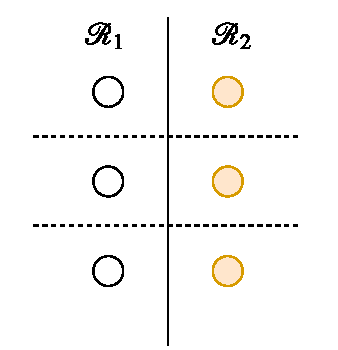
\includegraphics[width=0.35\linewidth]{fig/edit.pdf}
% 	\end{figure}
% 	\item [(b)] 串行剪辑算法的伪代码如下
% \begin{algorithm}
% \caption{串行剪辑算法}
% \begin{algorithmic}[1]
% \State 初始化$\mathcal{D}\gets$数据集,$n\gets$原型点个数
% \For{$\mathcal{D}$中每一个点$\vx_i$ ($i\gets 1$到$n$)}
% \If{$\vx_i$的最近邻与$\vx_i$同类}
% \State 从$\mathcal{D}$中移除$\vx_i$\Comment{否则保留$\vx_i$}
% \EndIf
% \EndFor
% \State\Return $\mathcal{D}$
% \end{algorithmic}
% \end{algorithm}

% 	考虑下面的例子,如果先处理$a$,则返回的$\mathcal{D}=\{b,c\}$;若先处理$b$,则返回$\mathcal{D}=\{a,c\}$。
% 	因此这种串行剪辑算法最后产生的结果依赖于样本点的处理顺序。
% 	\begin{figure}[H]
% 	\centering
% 	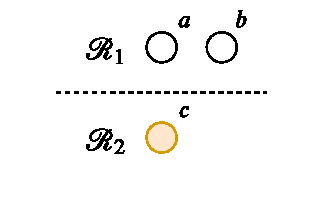
\includegraphics[width=0.3\linewidth]{fig/edit2.pdf}
% 	\end{figure}
% \end{itemize}
% \end{answer}

\begin{question}[\textsection 4 Q17]
考虑一种分类问题,总共有$c$个不同的类别,每一个类别的概率分布相同,并且每一个类别的先验概率都是$P(\omega_i)=1/c$。
证明公式(52)所给出的误差率上界
\[P\leq P^*\lrp{2-\frac{c}{c-1}P^*}\]
在本题中的“原信息”的场合下能够取到。
\end{question}
\begin{answer}
由题设有$p(\vx\mid\omega_i)=p(\vx),i=1,\ldots,c$,进而
\[p(\mathbf{x})=\sum_{i=1}^{c} p\left(\mathbf{x} \mid \omega_{i}\right) P\left(\omega_{i}\right)=\sum_{i=1}^{c} p(\mathbf{x} \mid \omega) \frac{1}{c}=p(\mathbf{x} \mid \omega)\]
而由条件概率
\[P\left(\omega_{i} \mid \mathbf{x}\right)=\frac{p\left(\mathbf{x} \mid \omega_{i}\right) P\left(\omega_{i}\right)}{p(\mathbf{x})}=\frac{p(\mathbf{x} \mid \omega) 1 / c}{p(\mathbf{x} \mid \omega)}=\frac{1}{c}\qquad(*)\]
将$(*)$式代入公式(45),有
\[\begin{aligned}
P &=\lim _{n \rightarrow \infty} P_{n}(e) \\
&=\int\left[1-\sum_{i=1}^{c} P^{2}\left(\omega_{i} \mid \mathbf{x}\right)\right] p(\mathbf{x}) \diff \mathbf{x} \\
&=\int\left[1-\sum_{i=1}^{c} \frac{1}{c^{2}}\right] p(\mathbf{x}) \diff \mathbf{x} \\
&=\left(1-\frac{1}{c}\right) \int p(\mathbf{x}) \diff \mathbf{x}=1-\frac{1}{c}
\end{aligned}\]

又将$(*)$式代入贝叶斯误差
\[\begin{aligned}
P^{*} &=\int P^{*}(\text {error } \mid \mathbf{x}) p(\mathbf{x}) \diff \mathbf{x} \\
&=\sum_{i=1}^{c} \int_{\mathcal{R}_{i}}\left[1-P\left(\omega_{i} \mid \mathbf{x}\right)\right] p(\mathbf{x}) \diff \mathbf{x}\\
&=\sum_{i=1}^{c} \int_{\mathcal{R}_{i}}\left(1-\frac{1}{c}\right) p(\mathbf{x}) \diff \mathbf{x}\\
&=\left(1-\frac{1}{c}\right) \int p(\mathbf{x}) \diff \mathbf{x}\\
&=1-\frac{1}{c}
\end{aligned}\]
因此有$P=P^*$,即误差率上界
\[P^*\lrp{2-\frac{c}{c-1}P^*}=1-\frac{1}{c}\]
在本题中的“原信息”的场合下能够取到。
\end{answer}

\end{document}